% to choose your degree
% please un-comment just one of the following
\documentclass[bsc,frontabs,twoside,singlespacing,parskip,deptreport]{infthesis}     % for BSc, BEng etc.
% \documentclass[minf,frontabs,twoside,singlespacing,parskip,deptreport]{infthesis}  % for MInf
\usepackage{cite}
\usepackage{graphicx}
\usepackage{float}
\usepackage{color}
\usepackage{xcolor}
\usepackage{ntheorem}   % for theorem-like environments
\usepackage{mdframed}   % for framing
\usepackage{csquotes}
\usepackage{amsmath}
\usepackage{amsmath}
\usepackage{tcolorbox}% http://ctan.org/pkg/tcolorbox
\usepackage{url}
\usepackage{tabularx}
\usepackage{subcaption}
\tcbuselibrary{skins}
\usetikzlibrary{shadings}
\begin{document}

\title{Temporal Ordering of Historical Events using Contextual Data}

\author{James Robert Friel}
% to choose your course
% please un-comment just one of the following
\course{Artificial Intelligence and Computer Science}
%\course{Artificial Intelligence and Software Engineering}
%\course{Artificial Intelligence and Mathematics}
%\course{Artificial Intelligence and Psychology }   
%\course{Artificial Intelligence with Psychology }   
%\course{Linguistics and Artificial Intelligence}    
%\course{Computer Science}
%\course{Software Engineering}
%\course{Computer Science and Electronics}    
%\course{Electronics and Software Engineering}    
%\course{Computer Science and Management Science}    
%\course{Computer Science and Mathematics}
%\course{Computer Science and Physics}  
%\course{Computer Science and Statistics}    
 
% to choose your report type
% please un-comment just one of the following
%\project{Undergraduate Dissertation} % CS&E, E&SE, AI&L
%\project{Undergraduate Thesis} % AI%Psy
\project{4th Year Project Report}

\date{\today}

\abstract{Meme Extreme}
%TODO


\maketitle

\section*{Acknowledgements}
Firstly I would like to thank my supervisor Shay Cohen for his guidance throughout the project.

I would also like to thank the ``School of Memeformatics'' group for assisting as a brain trust
throughout the project.

Thank you to Greggs Bakery for being there for me through thick and thin.

Lastly, thank you to Emily Wilson for her tireless proofreading and ability to put up with me.

\tableofcontents

%\pagenumbering{arabic}


\chapter{Introduction}
\section{The Problem}
In this project we investigate the effectivness of content from external data sources as aids to the temporal
ordering of events. Temporal ordering is defined as the arrangement of events in time.
The problem of ordering distinct events is not a new problem. There have been numerous papers published
in recent years on automatic ordering of events. These papers have typically worked on a single
topic domain such as cooking recipes or news articles. These related papers will be discussed further in Chapter~\ref{chapter:backgroundandrelatework}.
We intended to build on this work by
investigating if the reading of external data sources can aid in the temporal ordering of short
historical news article headlines.

Our event data comes from the ``Today in History'' data set from Mydatamaster~\cite{mydatamaster}. Each of these data points consists
of an event and a date such as
\begin{equation}
  [ \text{``Alaska becomes 49th State''}, \text{``1959-01-01''} ]\nonumber
\end{equation}


We tackled this problem through the use of summarising related articles and data of particular
events and determining their feasaility as aids to temporal ordering. 

\section{Aims \& Objectives}
The aim of this project was to experiment with machine reading on external data sources to
investigate the feasibility of extracting contextual data, from these sources, to aid in the
temporal ordering of historical events.

We aimed to do this by experimenting with machine reading techniques to extract the most
relevant contextual information from our data sources.

With this information, we intend to experiment with classification methods to optimise estimations
of singe edge ordering before generating a complete digraph from the resulting data.

Using the graph generated from our classifier, we attempted to find the optimum maximum spanning path
through every node by experimenting with various path finding techniques.
This path is the estimated ordering of history.


Using an evaluation metric, we discuss how the use of external data sources affects the system's ability to
temporally order events. Our methodology for the experiments conducted are discussed in detail in Chapter~\ref{chapter:methodology}

\section{Testing \& Evaluation}
With our data set of 6250 entries, it can
easily be split into training, development and testing with no
need for overlap. The data is split 80\% training,
10\% development and 10\% for testing.

Evaluation of the system was completed using the
Kendall rank correlation coefficient as it is a statistic
used to measure the ordinal association between two
measured quantities. This was applied to our results
by comparing the systems estimated ordering of events
with the label associated with the event from the data.
The results of these experiments and discussion of their meaning can be found in Chapters ~\ref{chapter:results} and ~\ref{chapter:discussion} respectively. 

\section{Implementation}
The experiments undertaken in this project consisted of Python and Bash scripts.
The following Python packages were used:
\begin{itemize}
\item Scikit-learn~\cite{scikit-learn} - Machine Learning tools for Python
\item Numpy~\cite{numpy} - package for scientific computation
\item Scipy~\cite{scipy} - Python library for scientific tools
\item Wikipedia~\cite{wikipediaAPI} - Python wrapper for integrating with Wikipedia's API
\item NLTK~\cite{nltk} - NLP toolkit for Python
\item Pool~\cite{pool} - Multiprocessing utility for Python
\item Pattern.en~\cite{pattern} - A web mining module 
\item Networkx~\cite{networkx} - Graph utility for Python
\item Matplotlib~\cite{matplotlib} - Visualisation tools
\item GenSim~\cite{rehurek_lrec} - Topic modelling for Python 
\end{itemize}
All classification and path-finding experiments were conducted using Python. A combination of
functions were built into the aforementioned packages, along with algorithms and function designed and implemented
specifically for the project.

Bash was used for automation of data sanitation and separating of the various data splits. 

Stanford's suite of NLP tools were used to perform information extraction on our data to provide the
object and relations of each event in order to gather article data from Wikipedia.
\section{Contributions}
While there has been a recent interest into temporal ordering of events, most papers discussing the topic focus on
ordering by using data already attributed to each event. Within this project we investigated the usefulness of
external data sources in aiding the ordering of short event texts. This was done through implementation
of article retrieval and relevancy, optimising classification of edge categorisation along withy construction and optimisation
of various pathing algorithms based on known theories and existing work. 
\chapter{Background \& Related Work}\label{chapter:backgroundandrelatework}
In this chapter we will discuss the current state of the research field relating to our project.
We will discuss in depth the topics of relation extraction and machine reading within a natural language understanding
context. Lastly, we will evaluate the current research and studies that relate to the work undertaken in this project.

\section{Relation Extraction}\label{sec:IE-bg}
Dependency parsing is the core of relation extraction.
By focusing on the dependencies between words, we can easily discover the relationships embedded within the text.
While there are numerous types of dependency representations, relation extraction is focused around semantic dependencies ~\cite{mcclosky2011event}.
Semantic dependencies are understood in terms of predicates and arguments.
\begin{figure}[H]
  \centering
  \includegraphics[scale=0.6]{semantic-dependancy.png}
  \caption{Example Semantic Dependency}
  \label{fig:semantic-dependancy}
\end{figure}

In the example semantic dependency in Figure~\ref{fig:semantic-dependancy} the two arguments \textit{John} and \textit{Football} are dependent
on the predicate \textit{likes}. This semantic dependency is the basis for relation extraction.


The information extraction (IE) techniques used to gather arguments and predicates for relation extraction use a combination
of well known natural language processing (NLP) techniques. 
Given a raw source text, IE typically follows a standard pipeline for entity extraction~\ref{fig:pipeline} ~\cite{bontcheva2013twitie}:\\
From the information gathered through IE, dependencies are build between the entities seen in the text
\begin{figure}[H]
\begin{tcolorbox}[width=\textwidth,
                  %%enhanced,
                  %%frame hidden,
                  interior hidden,
                  boxsep=10pt,
                  left=0pt,
                  right=0pt,
                  top=2pt]

 \begin{tabularx}{\linewidth}{lX}

 Language Identification &  Match source text language to known language footprints\vspace{1em}\\
  \multicolumn{2}{c}{$\Downarrow$} \\
 Tokenization &  Break input into a stream of word, phrases or other meaningful elements, called token\vspace{1em}\\

  \multicolumn{2}{c}{$\Downarrow$} \\
 Sentence Splitting &  Split tokens into discrete sentences\vspace{1em}\\

  \multicolumn{2}{c}{$\Downarrow$} \\
 Part-Of-Speech (POS) Tagging &   Assigns word tags, such as noun or verb, to each token\vspace{1em} \\

  \multicolumn{2}{c}{$\Downarrow$} \\
 Named Entity Recognition (NER) &   Either through handwritten rules or machine-learned NER recognising objects, such as a name or an
    organisation from the construction of word tags

 \end{tabularx}
\end{tcolorbox}
\caption{The Entity Extraction Pipeline}
\label{fig:pipeline}
\end{figure}


Historically, dependency parsing has consisted of only highly local models that extract each event and argument independently.
Modern techniques are building upon this to build systems that can handle more complex arguments. These systems use a tree of
event-argument relations represented in a re-ranking dependency ~\cite{mcclosky2011event}.
This system captures both flat relations, such as in Figure~\ref{fig:semantic-dependancy}, but also nested relations.
An example nested relation can be seen in Figure~\ref{fig:nested-relation}. These nested relations allow for more context to be drawn from
the source text.


\begin{figure}[H]
  \centering
  \includegraphics[scale=0.6]{nested-relation.png}
  \caption{Example Nested Relation}
  \label{fig:nested-relation}
\end{figure}


\section{Machine Reading}
The core aim of this project was to investigate the usefulness of Wikipedia article content as an aid to temporal ordering of events.
In order to perform this, we used machine reading on said articles.
Machine reading is the core problem of NLU.
NLU deals with machine reading comprehension, the problem of dissecting natural language inputs into usable features,
and is considered an AI-hard problem ~\cite{yampolskiy2012ai}.

Reading comprehension is the ability to read, process and understand text.  
There are two levels of reading comprehension, shallow (low-level) and deep (high-level).
Shallow comprehension involves structural and phonemic recognition along with the processing of sentence and  word
structure.
Deep comprehension involves semantic processing, which happens when we encode the meaning of a word and relate it
to similar words, this is fully discussed in Section~\ref{sec:word-embedding}.
This levels system of comprehension was first proposed by  Fergus I. M. Craik and Robert S. Lockhart ~\cite{wagner2009beyond}.
The ability to read and process text for all level of comprehension is built upon the IE pipeline discussed in Section~\ref{sec:IE-bg}.

One of the earliest known attempts at NLU by a computer was the STUDENT system in 1964 ~\cite{russell1995modern}.
Since then, NLU has become an
umbrella term for a diverse range of problems and applications. These applications range from simple tasks, such as
issuing simple commands to robots, to highly complex tasks such as full comprehension of poetry passages.
Most problems within NLU fit between these extremes and will implement one of the types of comprehension
depending on the task~\cite{bookman2012trajectories}.

Reading comprehension within these tasks is important. Applications, such as these, need not only understand the literal content
being passed to them, but also the contextual meaning within to better understand the nuances of the content.
Machine reading will be able to provide contextual information to provide better task performance when
involving unstructured data.

Unstructured data is data that has no pre-defined data model or manner. This type of data is
commonly seen in NLU with text mining and natural language rarely conforming to any cohesive model ~\cite{feldman2007text}.
From the data sources typically used with NLU (news articles or free-form speech and text) the unstructured format of
the data is beneficial as structured data typically has little contextual data ~\cite{feldman2007text}.
%Bit more about reading comprehension is CS

In recent years, there has been a commercial interest in NLU, mostly focusing on news-gathering, text categorising and
content-analysis. These systems vary vastly in terms of difficulty and use of comprehension. Some of the more
advanced techniques used within these systems include applying logical inference to the framework. This is often done
by mapping derived meaning into predicate logic, upon which logical deductions arrive at a conclusion.


\section{Related Work}
In recent years there has been an increasing interest in temporal ordering.
A number of different papers have been published on machine-learning approaches to temporal ordering of events.
Although there have been various different approaches to this problem, the most common and successful approaches typically
use unsupervised learning techniques. Typically, works often use pattern-based approaches and manually crafted rules ~\cite{chklovski2004mining}.  

Chambers and Jurafsky~\cite{chambers2009unsupervised} addressed unsupervised learning of event relations. Their evaluation
scenarios dealt with binary classification related to event ordering and aim to distinguish ordered sets
of events from random permutations. Along with this, their work on event structure and semantic roles will prove useful
to our work as external data sources can be riddled with synonyms and objects with similar attributes.
Their research into argument representation and semantic roles are a beneficial base
knowledge for our research into event extraction.
This argumentation representation consists of robust,
frame-specific roles about arguments. While frames are commonplace in NLP, the authors aimed to learn information
about the world without pre-defined frames, roles and corpora. This unsupervised learning of roles and frames could
be useful to our problem. Due to the nature of our data, structure and roles are not known prior to
IE. This representation also has the potential to assist in a variety of NLP applications ~\cite{chambers2009unsupervised}, which
we intended to build upon.

Abend et al. ~\cite{abend2015lexical} addressed the use of
edge-factor models in temporal ordering. The classification task we aimed to undertake is similar to that of ~\cite{abend2015lexical}
but with a significantly larger set of events to order.
Abend et al.~\cite{abend2015lexical} use a variation of the Hamiltonian path
to complete an integer linear programming ordering of their events. Along with this, their baseline is that of a greedy inference algorithm.
We looked at these two techniques as options for pathway estimation, but used a random assignment ordering as
a baseline. We chose to look at a random baseline as opposed to using greedy inference as
we wished to investigate the usefulness of greedy path-finding in comparison to an ILP approach.

Mani et al.~\cite{mani2006machine} discussed the use of both hand written and lexical rules for event tagging.
Their domain-independent approach to temporally anchoring and ordering events in the news is very accurate for both temporal
anchoring and partial ordering of events. Anchor events are time expressions which are normalised via
context, such as \textit{Last Tuesday}. Although we will not be building upon that papers work with
anchor events, it provides a good insight into the effectiveness of
partial orderings. We perform a total ordering without the use of anchored events, as described in this paper
as we wish to perfom unsupervised ordering of events.

While the methods discussed by Mani et al. ~\cite{mani2006machine} did not take into account dependencies between pairs of events, 
we see an alternative that does encompass
these dependencies in ~\cite{schapire1998learning}.
Schapire et al. discuses methods using greedy algorithms to approximate optimum rankings of objects.
It also discusses the use of ranking algorithms in the ordering of objects. The ranking methods discusses a
weakly-connected digraph and greedy ranking of said graph. This relates to our problem,
except we deal with strongly-connected digraph and investigated both greedy and ILP methods of finding
optimal solutions.


From the various paper discussed, temporal ordering of objects in any domain is of interest.
The use of argument and relation extraction from unstructured data has been discussed in numerous papers,
however none have yet succeded in the domain of unstructured, non-framed data.
There has been a significant improvement in recent years on the temporal ordering of events through the use of
directed graphs. We can see this from the use of ranking algorithms on weakly-linked
digraphs by Scapire et al.~\cite{schapire1998learning}, compared to Abend et al.'s ~\cite{abend2015lexical} use of edge-factor models in ordering predictions. 
%Should probably expand on each paper, advantages disadvantages etc

\chapter{Methodology}\label{chapter:methodology}
In order to evaluate the usefulness of an external data source, such as Wikipedia, we construct a methodology
for our experiments. We will discuss our choice of data set, extraction methods along with the reasoning behind the
classifiers and pathing methods chosen.
%Papers I have read and why we are doing this
%\section{Motivation}
%\section{Related Work}


%\section{The Data}%%Potential Chapter name change
%Intro to the data set
\section{Today In History Data set}
The Today In History data set we worked with consists of 6225 entries and is from Mydatamaster \cite{mydatamaster}.
Each entry consists of a  brief event title and the date in the form ``YYY-MM-DD''.
An example entry is
\begin{equation}
  \text{Alcatraz officially becomes a Federal Prison, 1934-01-01}\nonumber
\end{equation}
The data is a collection of events and has
an even distribution of events across the year (average 16.96 of events per day).

This data set was chosen as the events within are all objective historical events. This is beneficial as it minimised
any ambiguity when selecting Wikipedia articles to process. This, coupled with date labels already associated with
each event, made the data set favourable.


\section{Choice of External Data Source}
Wikipedia was chosen as the external data source for this project.
This is due to the nature of the events in our data set, historical points of note,
needing a source with a wide and deep range of articles.
As Wikipedia has over 5 million English language articles ~\cite{wikipediasize} and our original data
is taken from a Wikipedia outlet, we can assume
that most events are contained within its pages.


Wikipedia is also written in an reasonably unbiased, procedural manner wich alows more effective comprehension of events
than that of raw, unstructured data.
It is the key sentences within articles that we will use to estimate a timeline.

\section{Text Retrieval}\label{sec:retrieval}
Using Wikipedia's article retrieval Application Programming Interface (API) \cite{wikipediaAPI}, the task of gathering article content
from keywords in its title was trivial.

However, choosing what information is contextually relevant to the subject was not so straightforward.
Along with looking at how to extract the key entities and actions from our 
headlines, we also experimented with methods of extracting contextually relevant information from
retrieved articles related to the event headline.

\subsection{Information Extraction}\ref{sec:IE-bg}
Stanford's NLP suite,
a natural language analysis toolkit,
was selected to aid in extraction of features from the dataset.
Using this toolkit, the Open Information Extraction (OpenIE) from
the University of Washington was used to extract subjects, objects
and their relations from our event titles \cite{schmitz2012open}.


OpenIE implements a number of extraction techniques, such as noun-mediated extraction and N-ary extraction.
Noun-mediated extraction is an extraction technique where the predicate between the subject and object is a noun \cite{mirrezaei2015triplex}.
This is in constrast to N-ary extraction which extracts N length relations using a combination of the simpler extraction techniques, including noun-mediated \cite{akbik2012kraken}. 
We have seen through experimentation with the various extraction techniques that no method provided
usable relations for all inputs. Using OpenIE provided us with the ability to use multiple techniques and
use the best fitting results.

This system provided better relationship extraction than other systems available. Systems such as
ReVerb\cite{fader2011identifying} or WOE\cite{wu2010open} suffer from a few key weaknesses. These systems only provide verb mediated relation extraction \cite{schmitz2012open}.
This is problematic as sentences such as ``US President Donald Trump'' would not have the relation between \textit{US} and \textit{Donald Trump} extracted due to the structure of the relation lacking a verb.
These systems are also not built to use context for relation extraction and thus extract non-factual relations \cite{schmitz2012open}.
It is for these reasons that ReVerb and WOE were not chosen as our information extraction technique.


Along with OpenIE's ability to seamlessly use multiple extraction techniques to find the best available
relations for each event, it has numerous other properties that were beneficial to our project.
OpenIE is also useful as it does not require a schema specified in advance.
This is useful as we do not know the structure of the content that will be looked at.
This will allow the system to extract
more complex relationships, such as those seen in Figure~\ref{fig:compound-relations}, if such
a relationship can be found.


\begin{figure}[H]
  \centering
  \includegraphics[scale=0.4]{openie-train.png}
  \caption{Example of a compound relationship \protect\cite{OpenIE}}
\label{fig:compound-relations}
  \end{figure}

OpenIE can also deal more complex relations  than the simple relations.
It can look at positive or negative assertion within these relations.
This extra information may be beneficial to our solution as particular lenses are often applied to historical events.
It was these properties that made OpenIE the optimal system to extract the key relations from our events.


\subsection{Article Retrieval}
Using the objects and subjects generated by OpenIE we retrieved the relevant Wikipedia articles.
To do this we used fuzzy searching of Wikipedia, through their API, to get the articles relevant
for these objects and subjects.

Several different methods of extracting key sentences were experimented with.
These included:

\begin{enumerate}
  \item Extraction of only sentences that had a date within them
  \item Extraction of only sentences that had the other party in the relation within them
  \item Extraction of only sentences that had a date and the other party within them
  \item Extraction of paragraphs that referenced the other party
  \item Extraction of sentences that contained the object or the subject 
  \item Extraction of sentences that contained the object or the subject referenced the action between the two 
\end{enumerate}

As shown in Table~\ref{table:retrieval}, experimentation yielded mixed results.
The results show a large range of average number of sentences retrieved and varying degrees of relevancy.
Relevancy was measured manually using Cohen's Kappa (see Section~\ref{sec:cohen})\cite{wood2007understanding}.

Given that we wish to categorise our retrieved sentences into either related to the event, or not related,
we only have two possible categories to assign each of our N sentences to.

\begin{table}[H]
\centering
\begin{tabular}{|c|c|c|}
  \hline
Method & Average \# Sentences Retrieved & Relevancy \\
\hline
1      & 16                             &   -0.875  \\
2      & 2                              &   -1      \\
3      & 0.04                           &   0.5     \\
4      & 20                             &   -0.4    \\
5      & 27                             & -0.1\.{1}\\
6      & 32                             & 0.44\.{4}\\        
\hline
\end{tabular}
\caption{Retrieval Methods and their results}
\label{table:retrieval}
\end{table}

From these results, method 6 was chosen as our context extraction method.
While it doed not return the most relevant results, extraction method 3 did not provide
a sufficient number of sentences on average to build features.


Despite extraction method 6 not generating a perfect relevancy, under the time constraints
of the project, it was decided to move forward with the project rather than to incorporate more
complex solutions to improve relevancy.

%Link above to below section 
\subsection{Potential Issues With The Data Retrieved}\label{sec:dataIssues}
While we have seen positive attributes of Wikipedia, there are certain issues
that, if the content domain was to be altered, may cause an issue.

As Wikipedia is community managed, anybody can edit any page. This has been known to cause ``edit wars'' with users
uploading biased information about subjects \cite{hecht2009measuring}.
While in our current domain of long-term history, the facts and timelines are suitably coherent, if we were to apply this project
to a much more current or hotly contested subject - such as the O.J. Simpson trial, or 2016 presidential election - then Wikipedia
may not be the most appropriate source of information.
%Example


\section{Feature Extraction}\label{sec:representation}
Having extracted a series of sentences for each event in our data, we required a concise method
for representing these sentences. It is standard in NLP and machine learning domains to represent features as vectors.
Several different techniques were discussed, but ultimately due to time constraints only two methods were
experimented with: bag-of-words and word embedding.
\subsection{Bag-Of-Words}
The bag-of-words model is a simplifying representation of text.
In this model, we take a sentence, or multiple sentences, and represent them as a bag (multiset) of its words.
A multiset is similar to a set, but can allow multiple of the same item within.
For example, \{$\alpha,\beta$\} and \{$\alpha,\beta,\alpha$\} are the same set, but individual multisets.
This technique disregards grammar and order, but keeps multiplicity. It is a common technique in computer vision
and other learning situations \cite{sivic2009efficient}.

%Need to talk a bit more abput how we are making tuples of every event set
For our project, we implemented Bag-of-Words by using the relevant sentences for both of our events as a feature.
We chose to represent our multisets as counts over the vocabulary, so as to build numerical features to easily
use the data with classifiers. An example of the bag-of-words model can be seen in Figure~\ref{fig:bow}
%\newpage
\begin{figure}[H]
\begin{tcolorbox}[width=\textwidth,
                  %%enhanced,
                  %%frame hidden,
                  interior hidden,
                  boxsep=10pt,
                  left=0pt,
                  right=0pt,
                  top=2pt,
                  ]%%
  Given the sentences \vspace{0.5em}\\
  \begin{center}``John likes to watch movies. Mary likes movies too.''\\
  ``John also likes to watch football games.''\vspace{1em}\\
   \end{center}
    Based on these two text documents, a vocabulary list is constructed as follows:\vspace{1em}\\
    \begin{center}
  [``John'',``likes'',``to'',``watch'',``movies'',``also'',``football'',``games'',``Mary'',``too'']\vspace{1em}\\
\end{center}
    From this list a vector is constructed of the occurrences
    of each word across the sentences\vspace{1em}\\
 \begin{center} 
  Result: [2,3,2,2,2,1,1,1,1,1]
\end{center}
\end{tcolorbox}
\caption{An Example Bag-of-Words Usage}
\label{fig:bow}
\end{figure}

As bag-of-words only looks at single words at time and the contextual data may be lost through this method, we looked at
alternative methods to improve on this.

\subsection{N-Grams}
When experimenting with N-Grams, we tried to capture some of the meanings of phrases that appeared in the gathered
sentences.
This was achieved by looking for phrases and sequences of words that recurred throughout the sentences, under the assumption
that what reoccurs must be important. Due to the wide variety in the structure of the data we were seeing,
simple 2- or 3-Grams provided little to no use, returning junk phrases.

\subsection{Word Embedding}\label{sec:word-embedding}
Word Embedding was considered as this feature learning technique maps words or phrases to vectors of real numbers.
Advances in this method from Google in the past few years, such as the use of neural network architectures, have become
popular as methods to perform natural language processing (NLP) such as syntax parsing ~\cite{socher2013parsing}.

Using Gensim's Doc2Vec models \cite{rehurek_lrec}, we used this system to build thought vectors of our sentences.
Thought vectors are vectors made of whole sentences or documents, typically used in machine translation \cite{deeplearning4j}.
It was decided to use thought vectors as they correlate words with labels rather than word with words, which is done by bag-of-words.
This provides better representation of the words relating to ordering label, providing better results.

%Example of word embedding and such


From our experimentation, we discovered that thought vectors produced an accuracy 54\% less than that when
using bag-of-words. While this did not conform our hypothesis of using this technique, we believe
the main reason that word embedding did not perform as we expected was due to imperfect sentence retrieval causing noise in
the features. For this reason we did not move forward with word embedding beyond initial testing.

\section{Classifiers}\label{sec:classifiers}
\subsection{Decision Trees}
Decision trees were considered as they are a non-parametric, supervised learning method that are commonly used for
classification and regression.
They are based on the idea of asking simple yes/no questions. The algorithm is set up to be a binary tree with
each node being a question and each leaf a decision.

By inferring decision rules from data features, the system creates a model that predicts the value of a target variable.

These attributes were promising for our experiments as they fit with our data and generate
classifications of test data along with probabilities of these estimations.

%Some issues found with decision trees were that the probabilities generated were too narrowly distributed
%to infer any confidence in the paths generated. Due to this, it was decided to explore other methods of

\subsection{Support Vector Machines}
Similarly to decision trees, support vector machines (SVMs) provide supervised learning models based on
associated learning algorithms for classification and regression.

Given a set of labelled training data, an SVM will map this to a 3-D vector space.
When an unlabelled data point is inputted into the system, the SVM fits the new data into the vector space and
assigns  it to the closest vectors class.

%This proved beneficial as the results generated were better than the decision trees~\ref{table:local-learning}.
%SVMs also provided much better classification probability, which is favourable for path generation.
%\subsection{Linear Regression}
% To Be Completed in due course
%\vspace{4em}
\subsection{Logistic Regression}
Logistic regression was also experimented with as it utilises a binary dependent variable - that being where it
can only take one or two values, ``1'' or ``0'' in our case to represent correct ordering.


The logistic regression model estimates the probability of a binary response based on one or more independent features.
This is beneficial as along with providing classification estimates, the model can produce probabilities for its
decision. These probabilities allowed us to use weighting techniques to improve our path building.

\subsection{Perceptron}
The perceptron is a common algorithm used for large-scale learning.
It is a type of linear classifier that bases predictions on a linear predictor function that combines a set of optimised weights
and the input feature vector.
It is primarily used for supervised learning of binary classification.
This fit well with our data as the perceptron decides whether an input vector
corresponds to a specific class ~\cite{freund1999large}.

The perceptron model has several attributes that aided in improving the accuracy of our results.
These include:
\begin{itemize}
\item It does not require a learning rate.
\item It is not regularised (penalised).
\item It updates its model only on mistakes
\end{itemize}

Perceptrons allow retraining of the model when newer data is added, this allows the perceptron to
iteratively improve. An example of this improvement can be seen in Figure~\ref{fig:perceptronExample}.
It is these attributes that made the perceptron a suitable model to experiment with.
\begin{figure}[H]
  \centering
  \includegraphics[scale=0.7]{PerceptronExample.png}
  \caption{A diagram showing a perceptron updating its linear boundary as more training examples are added. \protect{\cite{goodspeed_2015}}}
\label{fig:perceptronExample}
\end{figure}

%For our experimentation, we trained the Perceptron model using  10 iterations with no regularisation term.
\subsection{Multilayer Perceptron}
Having discussed the use of Perceptrons, the next logical method to experiment with was multilayer perceptrons (MLP).
A Multilayer Perceptron is an feed-forward artificial neural network that maps the set of inputs
onto a set of appropriate outputs.
In Figure~\ref{fig:mlp} we see an example layer of an MLP.
An MLP consists of layers of  nodes in the form of a directed graph, with each layer connected to the next.
Each node, except the input node, is a neuron (processing element) with an activation function.%need a ref here
An activation function is a function that maps the weighted inputs of each processing element to an output.
MLPs are trained using backpropagation.

\begin{figure}[H]
  \centering
  \includegraphics[]{mlp-example.png}
  \caption{An Example one hidden layer MLP \cite{scikit-learn}}
  \label{fig:mlp}
\end{figure}

\section{Evaluation}
Throughout our experiments, there were several aspects that need to be evaluated.
The aspects that required measurment were:
\begin{itemize}
  \item Retrieved Sentence Relevancy
  \item Accuracy of Classifier
  \item Correlation of Predicted and True Path
\end{itemize}

There are multiple different statistics that were considered for each of these problems.
\subsection{Choice of Sentence Relevancy Metric}\label{sec:cohen}
In order to select a method to extract relevant sentences from Wikipedia, a statistic that measured the agreement
of relevancy was required. There are two main statistics for measuring inter-rater reliability: Cohen's Kappa and Fleiss' Kappa ~\cite{gwet2014handbook}.
These two statistics measure the agreement between reviewers. The main difference between Cohen's and Fleiss' Kappa is that
Cohen's Kappa only works for two reviewers, where as Fleiss' Kappa works for any number of fixed reviewers.
Given the short time frame of this project and availability of reviewers, it was decided to use Cohen's Kappa
to find an agreement between two reviewers selection of relevant sentences gathered from Wikipedia.

Cohen's Kappa measures the inter-rater agreement between two raters
who each classify N items into C mutually exclusive categories.

Cohen's Kappa is defined as:\\
\begin{equation}
  \kappa = \frac{p_{0} - p_{e}}{1 - p_{e}}\nonumber
\end{equation}

Where $p_0$ is the relative observed agreement between raters and $p_e$ is the hypothetical probability
of a chance agreement using the observed data to calculate the probabilities of each observer randomly assigning each category.

If the raters are in complete agreement then $\kappa$ = 1.
If there is no agreement among the raters, other than that expected by $p_e$, $\kappa \leq 0$.

Both statistics are thought to be a more robust measure than a simple percentage agreement.
This is because it takes into account the possibility of agreement occurring by chance.

\subsection{Choice Of Correlation Coefficient}\label{sec:kendall}

There are various, different correlation coefficients that could have be used to evaluate our generated pathways.
Some popular coefficients include:
\begin{itemize}
\item Pearsons Correlation Coefficient ( Pearson's r) - a measure of the strength and direction of the linear relationship between two variables
\item Intraclass Correlation - describes how strongly units in the same group resemble each other
\item Kendall Rank Correlation Coefficient -  measure of the portion of ranks that match between two data sets
\end{itemize}

For evaluation of our ordering, we decided to use the Kendall rank correlation coefficient (Tau coefficient).
This statistic was chosen as it can be used to measure the ordinal association between two measured quantities.
This allows us to evaluate what proportion of our ordering was correct, giving a truer representation of accuracy
compared to Pearson's r or Intraclass correlation~\cite{chok2010pearson}.
Pearson's r was not chosen as it measures the linear correlation between two variables.
This would not produce an accurate representation of the system as a single misaligned event would reduce the
correlation drastically.
Kendall's Tau was also preferred over Intraclass correlation as Intraclass correlation only quantifies the
degree to which two variables are related. This was of no value to the correlation of our estimated path
as this metic groups related items together.


The Tau coefficient is defined as
\begin{eqnarray}
  \tau=\frac{(\text{number of concordant pairs})-(\text{number of discordant pairs})}{n(n-1)/2}\nonumber
\end{eqnarray}\cite{abdi2007kendall}

The Tau coefficient was used as it measures results in terms of agreement in the range $-1 \leq \tau \geq 1$.
This allows us to show the agreement of our orderings, with 1 being a perfect agreement of the ordering, -1 being a perfect disagreement of the ordering and 0 claiming
total independence.


\section{Summary}
Throughout this section we have discussed the reasoning and methodology behind the project.
The use of our chosen data set, Today In History, was due to its large spread of events across
each day of the year. This should minimise bias to specific dates. The data also came with date labels and
consists of events outwith recent history, which aids in external data retrieval.

Discussing the benefits and drawbacks of using Wikipedia as an external data source found that
for our particular data set, historical events, bias in Wikipedia should not be of concern.
However, it was decided that if the project was to move into more recent history then this bias would
have to be discussed further.

Various, different article retrieval methods were discussed and tested.
Scoring each method on retrieved sentence relevancy, the methodology chosen provided acceptable relevancy
and a large enough corpus of sentences to be useful.

Also discussed were the advantages and drawbacks of the different feature extraction techniques and classification
techniques used within the project.

The different evaluation techniques used throughout the project were discussed and evaluated. 
For the task of sentence relevant, Cohen's Kappa \cite{wood2007understanding} was chosen as it measures the inter-rater agreement of
reviewers. Kendall's Tau \cite{abdi2007kendall} was chosen as the metric for measuring the correlation of our estimated ordering
against the true ordering of event. It was chosen as it measures the ordinal association between two
measured quantities rather than the linear comparison.


\chapter{Experiments}
For the methods discussed in Chaper~\ref{chapter:methodology} we required experimentation to optimise the classifiers.
In this Chapter, we will discuss how and why certain choices were made in regards to classifiers.
We will also discuss the Path-finding methods used to find the optimal path through the graph generated by the
classifiers.

\section{Classification}
In order to investigate if retrieved sentences aided in the  ordering of linear events we experimented with various
machine learning techniques to learn how to order events by sentences.
We aimed to determine if features generated from these important sentences provided a suitable training model
to improve orderings against a random assignment baseline. We then compared these features to the use of titles alone
to see if the use of retrieved sentences aids single edge ordering.


\subsection{Approach}\label{sec:approach}
A labelling technique was established to encode our data and train the classifier.

Given that each event in our data set is of the form:
\begin{equation}
  (t_{i},d_{i}) \hspace{0.5em} \text{for} \hspace{0.5em} i \hspace{0.2em}\in \hspace{0.2em} [M]\nonumber
    \end{equation}
    where t is the title, d is the associated date and M is the original data set,

    Using the Wikipedia extraction techniques discussed in Section~\ref{sec:retrieval} we constructed a new data set:
    \begin{equation}
      \{(t_{i},s_{i},d_{j})\} \hspace{0.5em} \text{for} \hspace{0.5em}i,j  \hspace{0.2em}\in \hspace{0.2em}[M]\nonumber
    \end{equation}
    Where $s_i$ is the sentences retrieved from Wikipedia for title $t_i$. 
    This formed the basis of our data to generate features.

    Using these sentences, we built a new data set
    \begin{equation}
      \{(t_{i},s_{i},t_{j},s_{j},b_{ij})\} \hspace{0.5em} \text{for} \hspace{0.5em} i,j \hspace{0.2em}\in \hspace{0.2em}[M]\nonumber
    \end{equation}
    where $b_{ij} = [y_{i} > y_{j}]$ indicates which event came first.\\
    We used this value as the label for our training data and to evaluate our results against.
    A similar data set was constructed using only the article headlines.
    
    From each of the entries in this new data set, we used the feature representation techniques discussed in Section~\ref{sec:representation} to build numerical
    features to train our classifier with.

Along with building a tuple event data set, we experimented with triple event entries.
\begin{equation}
      \{(t_{i},s_{i},t_{j},s_{j},t_{k},s_{k},b_{ijk})\} \hspace{0.5em} \text{for} \hspace{0.5em} i,j,k \hspace{0.2em}\in \hspace{0.2em}[M]\nonumber
\end{equation}

Where $b_{ijk} = [y_i > y_j > y_k]$ indicating if the ordering was correct for these events.

While we did not anticipate that increasing the dependency length of each entry would improve accuracy, it was investigated.
We anticipated that using more events per feature would diminish the accuracy of the system as
with a greater dependency tree, the availability of path transitions lessens~\cite{gerdes2013computational}.

As we expected, increasing the number of events associated with each training point greatly decreased the accuracy of results in all cases.
Due to this, we will not focus on discussing these experiments, but instead focus on the results gathered from the tuple data set.

We split our data set into 80\% for training, 10\% for development and 10\% for testing.
This breaks our 6226 entry data set into 4982, 622, 622 respectively.
The allotment of the entries into each category was done randomly.

Experimentation was done using the development set to optimise the parameters to give the most optimal results,
when finally tested on the testing data.
For each classifier, we fed in the training features and their associated label. These features were
be either the features generated from titles alone or with the sentences retrieved from Wikipedia.

Once training of the model was completed, we fed in a new data point without a class label.
The system returned a predicted class label for the new data and a probability score for its categorisation.

Each of these data points was similar to that of the training data
 \begin{equation}
   \{(t_{i},s_{i},t_{j},s_{j})\} \hspace{0.5em} \text{for} \hspace{0.5em} i,j \hspace{0.2em}\epsilon \hspace{0.2em}[M]\nonumber
 \end{equation}

 The classification returned for each data point was of the same style as that of the training data.
 %With these new data point classification we can begin to look at finding the optimal path through all of the nodes.
 %We will discuss the methods used in Chapter~\ref{chapter:graphing}.
 Each of the classification methods discussed in Section~\ref{sec:classifiers} required experimentation to optimise the
 parameters. Once optimisation of the parameters had occurred, we saw the best results from our classifiers.

 \subsection{Decision Tree}
 As Decision Trees infer decision rules from the training data provided to it, there were few parameters to
 experiment with. With our system being a binary classification system, there was no need to offset the class weightings.
 From this we did not require any parameters to be used when training the classification tree.
 
 \subsection{Support Vector Model}
 SVMs have the option of various parameters to be tune to optimise the results.
 In our implementation of an SVM we had the following parameters to experiment with:
 \begin{itemize}
 \item Penalty parameter of the error term
 \item The kernel type to be used in the algorithm
 \end{itemize}

 From experimentation with our development data, we found the optimal penalty parameter to be 1.0.
 This parameter indicates to the model how much you want to avoid classification of each example.
 Setting our penalty to 1.0 severely penalised the model for classification and lead to the model producing
 better results.

 SVMs use a kernel to turn a linear model into a non-linear model. This is beneficial as it allows the system
 to operate in high-dimensionality, implicit feature space without having to compute the coordinates of the feature
 in space \cite{hofmann2008kernel}.
 From our experimentation the Radial Based Function (RBF) kernel was chosen as it helps SVMs scale to large numbers of
 training samples which they do not typically perform well with.

 The RBF kernel for two same vectors, x and $\tilde{x}$, is defined as:
 \begin{equation}
   K_{RBF} (x, \tilde{x}) = \text{exp}[ \frac{||x =\tilde{x}||^2}{2\sigma^2}]\nonumber
 \end{equation}
\cite{hofmann2008kernel}
 This kernel can project into infinite dimensions and therefore allows for easy computation of new coordinates, as
 we have a high number of training samples.
 
 \subsection{Logistic Regression}\label{sec:log-reg}
 When using the Logistic Regression model, there were only a few parameters that were of interest:
 \begin{itemize}
   \item Type of penalty
   \item Type of solver
 \end{itemize}

 There are two main types of penalties that can be applied to Logistic Regression models, L1 and L2 loss functions.
 L1, also known as  the least absolute deviations, is a loss function that minimises the sum of of the absolute
 differences (S) between the target ($Y_i$) and the estimated values ($f(x_{i})$) \cite{l1l2}.
 \begin{equation}
   S = \sum_{i=1}^{N} | Y_i - f(x_i)|\nonumber
   \end{equation}
 
 L2 is also known as least square error. It minimises the sum of the square of differences (S) between
 the target ($Y_i$) and the estimated values ($f(x_{i})$) \cite{l1l2}.
 \begin{equation}
   S = \sum_{i=1}^{N} ( Y_i - f(x_i))^2\nonumber
   \end{equation}

 L2 was chosen as it always provides a single, stable solution where as L1 can return multiple solutions
 which is of no use for our system.

 There are several different solvers that can be effectively used with a Logistic Regression model.
 For our system, we chose to use the LIBLINEAR solver as it supports L2, provides probabilities
 for Logistic Regression and is a linear classifier for large data sets\cite{fan2008liblinear}.
 
 \subsection{Perceptron}
 During our experimentation with Perceptron parameters, we discovered that giving the system nine epochs (passes
 over the training data) and shuffling the training data on each iteration provided results that maximised the
 estimations. For the same reasons stated in Section~\ref{sec:log-reg}, we used an L2 penalty with our perceptron
 model.
 
 \subsection{Multilayer Perceptron}
 In order to effectively use an MLP for our data we experimented with various parameters.
 \begin{itemize}
 \item Number of hidden layers - the number of neurons per layer
 \item Type of activation function
 \item Type of solver
 \item L2 penalty
 \item Maximum number of iterations
 \end{itemize}
 
 After running experiments on  small subsets of our data, we found the optimal number of hidden layers to be 100. 
 This aids the model in transforming the inputs into appropriate information for the output layer.
 
 Having looked at logistic and identity activation functions, the rectifier activation function was chosen.
 The rectifier activation function is the most popular activation function \cite{lecun2015deep} and is defined as
 \begin{equation}
   f(x) = \text{max}(0,x)\nonumber\\
 \end{equation}
 Where x is the output of a neuron.
 
 The rectifier function was chosen as it is more effective than its available counterparts~\cite{glorot2011deep}.

 In order to solve the weight optimisation, we used the Broyden-Fletcher-Goldfarb-Shanno (BFGS) algorithm.
 This algorithm was chosen as it is an iterative model for non-linear optimisation.
 An L2 penalty of 0.00005 was chosen to aid our model beyond the training data.
 We chose the value of 0.00005 so as to prevent division by zero. 

 The last parameter we experimented with was the number of epochs.
 100 layers were chosen as during experimentation with subsets of the data improvements were
 insignificant.

 \section{Path Finding} \label{chapter:graphing}
From our classifier, we constructed a directional ordering between every two events.
Each of our events was represented by a node and placing each individual ordering on an edge, we constructed
a digraph of the data.
A digraph is an ordered pair G = (A,V) where~\cite{bang2008digraphs}
\begin{itemize}
  \item V is the set of nodes
  \item A is a set of ordered pairs of vertices
\end{itemize}
An example of such a graph can be seen in Figure~\ref{fig:digraph}.

It was with this new graph that we began to experiment with methods to construct the most probable path through every
node in the graph.


\begin{figure}[H]
  \centering
  \includegraphics[scale=0.5]{ExampleDigraph.png}
  \caption{A small example of our results placed in a digraph}
  \label{fig:digraph}
 \end{figure}

\subsection{Travelling Salesman Problem}
The Travelling Salesman Problem (TSP) is a  NP-hard algorithm problem~\cite{junger1995traveling}.%something about NP hard problems
It is defined as
\begin{center}
\enquote{A travelling salesman wants to visit each of a set of towns exactly once, starting
from and returning to his home town. One of his problems is to find the shortest
such trip}~\cite{junger1995traveling}
\end{center}

While the TSP algorithm is still unsolved, we fortunately only had to solve a a modified version of the problem.\\

\begin{center}
  \enquote{Given a graph with directed edges, find the optimal path from some starting node through all other nodes in
  the graph.}
\end{center}

These restrictions on the graph made finding an optimal path through the graph simpler.


\subsection{Pathing Algorithms}
There have been numerous algorithms developed to find the shortest and longest paths through various types of graphs.
As we required a total traversal of our graph, several of these algorithms were eliminated.

In order to accommodate many shortest-path algorithms, a new graph was constructed with edge weights between nodes being inverted,
$\frac{1}{W}$ where W is the edge weight. This allowed paths that look for the cheapest path to be usable as they will traverse the
true most expensive path, which will encompass all nodes.

There are two main types of solutions to optimal pathing: Greedy and Integer Linear Programming.
We will discuss the options available in each type of solution and the benefits there in.

\subsection{Greedy Solution}
A greedy algorithm is an algorithm that follows the problem solving heuristic of making locally optimal choices at each stage with the aim
of finding a global optimum~\cite{black2004dictionary}.
While a greedy strategy does not in general produce a global optimum, it may produce locally optimum solutions that approximate a globally optimum solution.


The greedy strategy for our variation of the travelling salesman problem was the following heuristic:
``At each stage, visit an unvisited city nearest to the current city.''\\
Where nearest is defined as the lowest edge-weight.


%Need some beam search refs
The greedy algorithm used was beam search.
It was chosen as it follows the greedy heuristic and also stores partial orderings,
allowing us to prune solutions that do not cover all nodes.
An example of this pruning ability can be seen in Figure~\ref{fig:beam-prune}.

\begin{figure}[H]
  \centering
  \includegraphics[scale=0.5]{BeamSearchPruning.png}
  \caption{An Example of beam search prunining\\ Iteration 1: Blue Iteration 2: Green, Iteration 3: Yellow}
  \label{fig:beam-prune}
\end{figure}

As we did not know the optimal starting node, we executed our greedy solution from each of the event nodes.
Due to every edge of graph being directional, it was possible that for any given starting node, that a solution for traversal
of every node is impossible. To counteract this, and allow every node to generate a full path, a penalty system was implemented.
This penalty system worked by allowing a path to deviate from any edges classified direction given that all other path options
were exhausted. This deviation cased a large penalty to be applied to the path and typically rendered the paths start node
unfeasible as a potential true starting node. 

With this we generated the optimal greedy path through our graph. The results of which can be seen in Section~\ref{sec:graph-results}.

\subsection{Integer Linear Programming Solution}
Integer Linear Programming (ILP) is a mathematical optimisation where the objective function and the constraints are linear.
ILP is common in the field of optimisation and is ideal for our needs. ILP aims to find the globally most optimal solution using global interence.
Global Inference produces the best global solution by inferring predictions from each input~\cite{roth2004linear}.%More here
When applied to path-finding ILP should generate the best global path through all nodes, rather than finding the next most optimal node like in a greedy solution.


The A$*$ search algorithm is a special case of the generalisation of branch and bound~\cite{balas1983branch} and is derived from the primal-dual algorithm for ILP~\cite{ye2012note}.
We chose this algorithm as it follows the ILP methodology. The algorithm works similarly way to best-first search, but takes into account the path cost already travelled.
This was beneficial as it will give us the globally optimum path by finding the most probable total path, rather than the most probable next step when using a
greedy algorithm. We can see an example of the complete digraph and the estimated path through it in Figure~\ref{fig:minigraph} and ~\ref{fig:minigraph-clean}.
Similarly to the greedy solution, as we do not know the optimal start and end node, we had to run the algorithm with every possible start and end node combination.
\begin{figure}[H]
\centering
  \centering
  \includegraphics[width=\textwidth]{node-graph2.png}
  \caption{An example graph generated using 10 events, where each edge direction is indicated by a block head. Red edges indicate estimated path}
  \label{fig:minigraph}
\end{figure}
\begin{figure}[H]
  \centering
  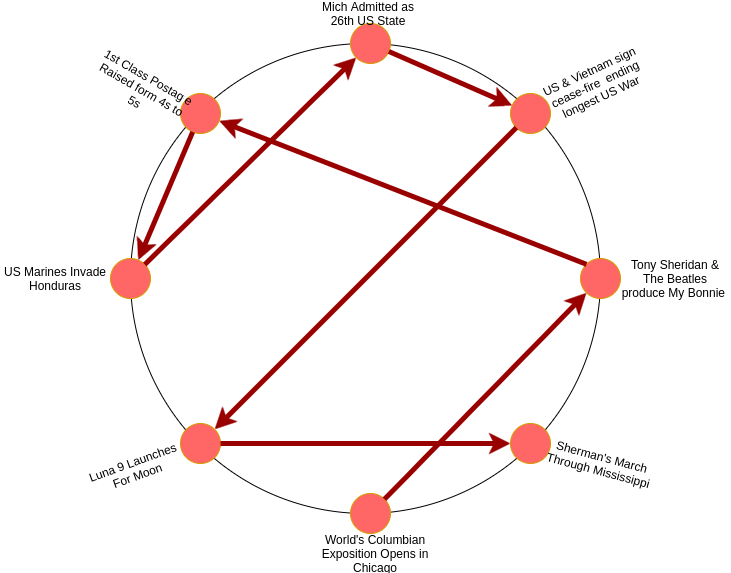
\includegraphics[width=\textwidth]{node-graph.png}
\caption{The example graph from Figure~\ref{fig:minigraph} with only the estimated path shown }
\label{fig:minigraph-clean}
\end{figure}

\section{Summary}
In this chapter we have discussed the experiments carried out within this project.
We also discussed the approach taken to adapting our data to allow classification of event pairs. This involved building a new data set
in which each entry consisted of two events. This was done for each entry with every other entry, from which a complete
graph can be constructed.

Also discussed was the experimentation with parameters for each classifier to maximise the results. This was done through
testing of penalties, solvers and kernel type among others.

The various different path-finding methods for the graph generated from the data was also discussed.
We looked at both ILP and Greedy solutions to the problem.

\chapter{Results}\label{chapter:results}
In this chapter we report the results gathered from our experiments dicussed previously.
We look at both classifcation and path-finding results along with measurements about the data gathered.
From our experiments, results were generated from both our classification and path-finding methods.
Given the spread of results from our classification of tuples and triples of events, we used both of our path finding
techniques in each of the resulting graphs. Our results include accuracies and correlations from
experiments using both the sentences extracted from Wikipedia and just the event titles alone.   

\section{Classification}
The results of edge classification between both two and three events can be seen in Tables~\ref{table:classification-results}
and~\ref{table:triple-classification-results} respectively. The results of these tables in measured by the
proportion of true results, both positive and negative, among the total number of results.

The baseline used for classification is a random assignment.
As each classification made is a binary value along a single edge between events, each classification has a
50\% chance of correct classification because we do not apply class weights.
Given that each classification of triple sets requires two edges (A $\rightarrow$ B $\rightarrow$ C) the probability of a correct
classification is 0.25\%. By applying this across the whole graph, the random assignment of edge classification yields an
accuracy of
\begin{equation}
\frac{1}{4^N} \nonumber
\end{equation}
Where N is the number of nodes in the graph.
Given that our results are based on 622 events, the baseline accuracy for triple set events is $\frac{1}{4^{622}}$.

The results generated using triple sets of events per classification report such poor accuracy with
(mean = 19.4, standard deviation = 6.22896) or without articles (mean = 20.6, standard deviation = 8.61972). These poor results, regardless of use of article data,
conform with our original hypothesis in Section~\ref{sec:approach}. 


The baseline for tuple of events is similar to that of the triples, but as each classification only requires one edge
the random assignment accuracy is
\begin{equation}
  \frac{1}{2^N}\nonumber
\end{equation}
Where N is the number of events.
Given our 622 test events, the accuracy is $\frac{1}{2^{622}}$.


From our results generated using tuples of events, we can see that classification using only the event titles
have a small spread of results (mean = 47, standard deviation = 15.09).
Our experiments that used the retrieved sentences out-perform the results using only titles by large margins.
These experiments are centred around 66 and have a much lower spread that with the use of titles alone
(mean = 65.\.{3}, standard deviation = 12.1)

\begin{table}[H]
\centering
\begin{tabular}{|c|c|c|c|c|c|c|c|}
  \hline
  Accuracy  & DT  & SVM & LR & Perceptron & MLP & Baseline\\
  \hline
  With Articles    & 53\%   & 66\% &  76\% & 66\% & 83\% & $\frac{1}{2^{622}}$\%\\
\hline
With Titles & 43\%  & 51\%    & 52\% & 46\% & 54\% & $\frac{1}{2^{622}}$\%\\
\hline
\multicolumn{3}{@{}p{1.5in}}{\footnotesize DT $=$ Decision Tree}\\
\multicolumn{3}{@{}p{1.5in}}{\footnotesize LR $=$ Logistic Regression}\\
\multicolumn{3}{@{}p{2in}}{\footnotesize MLP $=$ Multilayer Perceptron}\\
\end{tabular}
\caption{Classification Results for Tuples}
\label{table:classification-results}
\end{table}


\begin{table}[H]
\centering
\begin{tabular}{|c|c|c|c|c|c|c|}
  \hline
  Accuracy  & DT & SVM & LR & Perceptron & MLP & Baseline\\
  \hline
  With Articles & 13\%    & 13\% &  23\% & 27\% & 21\% &  $\frac{1}{4^{622}}$\%\\
\hline
With Titles & 21\% & 13\%    & 24\% & 33\% & 14\% &  $\frac{1}{4^{622}}$\%\\
\hline
\multicolumn{3}{@{}p{1.5in}}{\footnotesize DT $=$ Decision Tree}\\
\multicolumn{3}{@{}p{1.5in}}{\footnotesize LR $=$ Logistic Regression}\\

\multicolumn{3}{@{}p{2in}}{\footnotesize MLP $=$ Multilayer Perceptron}\\
\end{tabular}
\caption{Classification Results for Triples}
\label{table:triple-classification-results}
\end{table}


\section{Path Finding}\label{sec:graph-results}
As discussed in Section~\ref{sec:kendall}, our path finding results were measured using Kendall's Tau.

Our baseline for the generated paths is zero when using Kendall's Tau.
This is due to when randomly ordering a set of data it will, on average, score a zero against the true ordering
when using Kendall's Tau.


From the use of ILP path-finding method, we gathered the results for tuples of events in Table~\ref{table:ILP-results}.
As we can see, the use of articles greatly increases the correlation of estimated path with the true path.
These results have a much smaller spread (mean = 0.50466 , standard deviation = 0.1756) than the ILP pathing of titles alone
(mean = -0.1, standard deviation = 0.219).

\begin{table}[H]
\centering
\begin{tabular}{|l|l|l|l|l|l|l|l|}
  \hline
  A$*$ Search & DT & SVM &LR & Perceptron & MLP & Baseline\\
  \hline
With Articles & 0.695 & 0.419 & 0.3 & 0.376   & 0.7333  & 0\\
\hline
With Titles &0.06  & -0.09 & 0.048 & -0.52  & -0.28 & 0\\
\hline
\multicolumn{3}{@{}p{1.5in}}{\footnotesize DT $=$ Decision Tree}\\
\multicolumn{3}{@{}p{1.5in}}{\footnotesize LR $=$ Logistic Regression}\\
\multicolumn{3}{@{}p{2in}}{\footnotesize MLP $=$ Multilayer Perceptron}\\
\end{tabular}
\caption{ILP Pathing Results for Tuples}
\label{table:ILP-results}
\end{table}

Using the greedy solution to path-finding, we found our results to have a much lower spread
than the ILP results (mean = 0.46, standard deviation = 0.05) when using article data.
Our results in Table~\ref{table:greedy-results} indicate that once
again, using article data aids in the ordering correlations of estimated paths rather than when just using event tiles.
The results from just event tiles shows no significant difference to that of the ILP results
(mean = 0.0348, standard deviation= 0.3357).

\begin{table}[H]
\centering
\begin{tabular}{|l|l|l|l|l|l|l|l|}
  \hline
  Beam Search & DT & SVM &LR & Perceptron & MLP & Baseline\\
  \hline
With Articles & 0.42 & 0.5151 & 0.3 &  0.44  & 0.5454  & 0\\
\hline
With Titles & 0.214 & -0.62 & 0.17 & 0.09  & 0.32 & 0\\
\hline
\multicolumn{3}{@{}p{1.5in}}{\footnotesize DT $=$ Decision Tree}\\
\multicolumn{3}{@{}p{1.5in}}{\footnotesize LR $=$ Logistic Regression}\\

\multicolumn{3}{@{}p{2in}}{\footnotesize MLP $=$ Multilayer Perceptron}\\
\end{tabular}
\caption{Greedy Pathing Results for Tuples}
\label{table:greedy-results}
\end{table}

With the use of triples of events, pathing in either greedy or ILP prove fruitless. The results seen in Table
\ref{table:greedy-results-triples} confirm our hypothesis that longer event dependencies are detrimental to the
accuracy of the system. The use of Articles (mean= -0.642, standard deviation= 0.16131) shows no significant difference from
the use with just titles (mean= -0.674,standard deviation= 0.11459) with both results falling far below that of the tuples of events.


\begin{table}[H]
\centering
\begin{tabular}{|l|l|l|l|l|l|l|l|}
  \hline
  A$*$ Search & DT & SVM &LR & Perceptron & MLP & Baseline\\
  \hline
With Articles & -0.64 & -0.54 & -0.92 & -0.53   & -0.58  & 0\\
\hline
With Titles & -0.62  & -0.68 & -0.87 & -0.61  & -0.59 & 0\\
\hline
\multicolumn{3}{@{}p{1.5in}}{\footnotesize DT $=$ Decision Tree}\\
\multicolumn{3}{@{}p{1.5in}}{\footnotesize LR $=$ Logistic Regression}\\
\multicolumn{3}{@{}p{2in}}{\footnotesize MLP $=$ Multilayer Perceptron}\\
\end{tabular}
\caption{ILP Pathing Results for Triples}
\label{table:ILP-results-triple}
\end{table}


\begin{table}[H]
\centering
\begin{tabular}{|l|l|l|l|l|l|l|l|}
  \hline
  Beam Search & DT & SVM & LR & Perceptron & MLP & Baseline\\
  \hline
With Articles & -0.81 & -0.73 & -0.96 & -0.73   & -0.69  & 0\\
\hline
With Titles & -0.81  & -0.79 & -0.9 & -0.74  & -0.68 & 0\\
\hline
\multicolumn{3}{@{}p{1.5in}}{\footnotesize DT $=$ Decision Tree}\\
\multicolumn{3}{@{}p{1.5in}}{\footnotesize LR $=$ Logistic Regression}\\
\multicolumn{3}{@{}p{2in}}{\footnotesize MLP $=$ Multilayer Perceptron}\\
\end{tabular}
\caption{Greedy Pathing Results for Triples}
\label{table:greedy-results-triples}
\end{table}


\chapter{Discussion \& Further Work}\label{chapter:discussion}
In this chapter we will discuss the results gathered and what this means in terms of our project goals.
We will also discuss potential improvments that could be made to the system as a whole under further work.
\section{Discussion}
%discuss wikipedia retrieval
%%%
%Discuss how triples are shit and why
%Wont talk about those, only tuples
%Discuss various classifiers and why they were good
%Talk about overall how the pathing methods were good/bad
%Discuss in detail the best 2(?) overall results and what this means
%%%
As We can see from Tables~\ref{table:triple-classification-results}, ~\ref{table:greedy-results-triples} and
~\ref{table:ILP-results-triple} our original hypothesis, outlined in Section~\ref{sec:approach}
involving the use of triples of events holds true.
These results confirm that performing edge classification on three events, per edge, greatly reduces the
accuracy of classification and subsiquent path-finding. This is due to the dependency of each edge
increasing with each node added and as the dependency increases the likelyhood of total success lessens \cite{gerdes2013computational}.

These results are eclipsed by the those seen in Tables~\ref{table:classification-results}, ~\ref{table:ILP-results} and ~\ref{table:greedy-results} with the use of tuples of events.
Due to these reults being unequivocally better than those using tuples of events, we will focus our discussion from here on
the results generated by tuples off events.

As we see in  Tables~\ref{table:ILP-results} and~\ref{table:greedy-results}, the use of event titles alone
provides a poor classification, centred around roughly 50\% accuracy. This may be due to a number of reasons,
but the key factor on these results is the lack of strong features to learn from. With each event title having an average of
8.24 words, the features generated are typically  sparse. We believe this is the main reason that ordering using
only title information is so poor.

The varying results of Table ~\ref{table:classification-results} show a wide spread of accuracies between the classifiers.
Both with and without article data, the classifiers follow the same trends of accuracy
\begin{equation}
\text{MLP $\Rightarrow$ Logistic Regression $\Rightarrow$ SVM $\Rightarrow$ Perceptron $\Rightarrow$ Decision Tree }\nonumber  
\end{equation}
With the orderings going from highest to lowest accuracy.

The results are interesting for several reasons.
It is unusual for SVMs to perform better than Decision Tree Classifiers, in our situation this may be due to the chosen
kernel for the SVM performing linear decision boundaries very well. Decision trees, while simple, may misidentify the important
aspect of a  feature, in retrospect it may have been useful to look at additive trees, such as MART~\cite{friedman2001greedy}, in order to
improve upon these results.
We also note that the use of a single Percpetron is vastly worse than the use of a MLP, this is as expected as
the properties of an MLP typically provide better results than that of a single Percepton.
These results for the various classifiers used are as expected, with Logistic Regression and MLP performing the best
at edge classification. Logistic Regression perfored well due to its ability to deal with linear categorical data.
While Logistic Regression performed well at the task, MLP overshadowed these reults with it's significantly higher
accuracy. 


Overall, the ILP pathing solution out performed the Greedy solution. This was to be expected as greedy pathfinding can
approximate an ILP under favourable conditions ~\cite{schapire1998learning}. We can see from Table~\ref{table:ILP-results} that the
correlation accuracies do not align perfectly with the classifier accuracies, notably with Logistic Regression moving
down the rankings. We believe this reordering of most accurate classifiers is due to the pathing algorithms misaligning
sections of the true ordering. An example of this being:
\begin{align}\nonumber
  \text{Generated Order : 1 2 3 6 7 8 4 5 9}\\\nonumber
  \text{True Order : 1 2 3 4 5 6 7 8 9}\\\nonumber
  \text{Where each number is an event}\nonumber
\end{align}

As we can see from this example, the generated order will place a small number of ordered events (6,7,8) earlier or
later in the path. This is due to an incorrect edge direction with a high probability and relates back to the
inaccuracies in our classifiers. It this these sort of issue that cause the reordering of prefered methods when considering
path optimisation.

The most accurate results come from the Decision Tree Classifer and the Multilayer Perceptron classifier.
Both of these method, using an ILP solution, prove very strong result corelations. This show that, despite there
being room for improvement within the experiments, the use of external data sources does aid in the temporal ordering
of historical events.

\section{Further Work}
While the work done in this project does confirm the validity of aiding temporal ordering through the use of contextual
data, there are several aspects that could be improved upon and various methodologies that could be explored, given further
time.

\subsection{Improvement Of Relevant Sentence Retrieval}
In Section~\ref{sec:retrieval} we discussed various possible sentence extraction techniques.
While the relevant and number of sentences extracted was suitable for our purpose, there was certainly room for improvement.

In order to improve the relevancy of sentences extracted, we would suggest exploring the following avenues:
\begin{itemize}
\item Implementing Semantic Sentence Trimming, a method discussed by Zajic et al.~\cite{zajic2005sentence} that
  uses linguistic-motivated heuristics to remove low content syntactic constituents 

\item The use of inter-sentence relevance instead of similarity of content may provide a potential improvement of
  overall sentence retrieval relevancy. We would suggest that this method be based upon the work of Zhong et al~\cite{zhong2008practical}
\end{itemize}

\subsection{Potential Extension of Data Retrieval}
As we discussed in Section~\ref{sec:dataIssues}, while Wikipedia has a large catalogue of articles to extract from,
it does have several points that may be an issue if this project was to be taken further.

These issues include potential bias in information due to Wikipedia's open editing rules~\cite{wikipediaeditrules}. The current lack of
cross-referencing is also a potential issue as cross-validation of timelines would further reinforce the knowledge acquired.
It is with this in mind that we would suggest, if this project was to be changed to deal with more developing stories, that
multiple sources of information be investigated with cross-referencing between these sources to build a stronger picture of
the events.


\subsection{Use Of Global Learning Methods}
In this project we have explored methods involving single edge classification. Given more time,
this project could be advanced through the use of techniques discussed by Abend et al.~\cite{abend2015lexical}.
In this paper they discuss the application of global learning on temporal ordering problems. Global learning
fits a distribution over the data. This methodology learns the parameters from observations of the data~\cite{Huang2008}
and has the potential to make vast improvements on this work thus increasing the validity
of external contextual data on temporal ordering. It is with this in mind that using global learning techniques on the problem
would be strongly suggested in the future.

\subsection{Comparison of Path-finding Techniques}
In this project, we considered both ILP and greedy solutions to optimal path-finding through the generated graphs.
The implementations of algorithms were not optimal. Looking further into both ILP and greedy solutions would
be recommended as while ILP typically outperforms Greedy, the runtime of our ILP solution is more computationally
expensive. Greedy algorithms have been shown to provide approximations that come close to ILP solutions under the right
conditions, with much lower cost, as shown in Schapire's paper~\cite{schapire1998learning}. With this in mind,
it such a solution should be investigated for our problem. If this method can
be applied to the problem of temporally ordering events, then the scale of events considered could be greatly increased with
an improved runtime.

%This potential improvement could also lead into other ability of reordering based on new information.
%Discuss news articles as they apear


\chapter{Conclusion}
As we have seen thoughout our experiments, the usefulness of external data in aiding the temporal ordering
of historical events is valid. We have seen that the use of this external content can impove accuracies by up to
30\% over the use of event headline alone.
Article retrieval and relevent sentence extraction proved to substantialy aid in the temporal ordering of events.
The methods discussed, in combination with experimentation with classification models, performed substantially better
than using data from event titles only.
The various classification methods used show this trend with varying success. Using multilayer Perceptrons provided an
imporved accuracy of 30\% with article usage over titles alone, boasting 83\% accuracy compaired to 54\% when using titles
alone.


These results are not the ceiling for this subject area, methods and approaches discussed in this paper have scope
to be improved upon. The use of Wikipedia as an external source of content has been proven as a valid source for
long term historical, but may pose issues if applied to recent history. Overall, we have shown that the use of external
data sources, such as Wikipedia, do aid in the temporal ordering of historical events and provide a promising base for future
research into this domain.
% otherwise generate bibtem entries
\bibliographystyle{plain}
\bibliography{./references.bib}
\end{document}
